\newcommand{\fieldsize}{22pt}
\begin{figure}[t]
  \centering
  \begin{subfigure}[b]{0.15\textwidth}
    \setlength{\tabcolsep}{2pt}
    \begin{tabular}{cc}
      \tcbincludegraphics[size=tight,hbox,graphics options={width=\fieldsize}]{figures/sim-real-gabors/ringach/1-real.pdf} &
      \tcbincludegraphics[size=tight,hbox,graphics options={width=\fieldsize}]{figures/sim-real-gabors/ringach/5-real.pdf} \\
      \tcbincludegraphics[size=tight,hbox,graphics options={width=\fieldsize}]{figures/sim-real-gabors/ringach/2-real.pdf} &
      \tcbincludegraphics[size=tight,hbox,graphics options={width=\fieldsize}]{figures/sim-real-gabors/ringach/6-real.pdf} \\
      \tcbincludegraphics[size=tight,hbox,graphics options={width=\fieldsize}]{figures/sim-real-gabors/ringach/3-real.pdf} &
      \tcbincludegraphics[size=tight,hbox,graphics options={width=\fieldsize}]{figures/sim-real-gabors/ringach/7-real.pdf} \\
      \tcbincludegraphics[size=tight,hbox,graphics options={width=\fieldsize}]{figures/sim-real-gabors/ringach/4-real.pdf} &
      \tcbincludegraphics[size=tight,hbox,graphics options={width=\fieldsize}]{figures/sim-real-gabors/ringach/8-real.pdf} \\
      \multicolumn{2}{c}{\scriptsize\parencite{ringach2002spatial}}
    \end{tabular}
  \end{subfigure}
  \begin{subfigure}[b]{0.09\textwidth}
    \setlength{\tabcolsep}{2pt}
    \begin{tabular}{cc}
      \tcbincludegraphics[size=tight,hbox,graphics options={width=\fieldsize}]{figures/sim-real-gabors/decharms/fig2-d.pdf} \\
      \tcbincludegraphics[size=tight,hbox,graphics options={width=\fieldsize}]{figures/sim-real-gabors/decharms/fig2-e.pdf} \\
      \tcbincludegraphics[size=tight,hbox,graphics options={width=\fieldsize}]{figures/sim-real-gabors/decharms/fig2-f.pdf} \\
      \tcbincludegraphics[size=tight,hbox,graphics options={width=\fieldsize}]{figures/sim-real-gabors/decharms/fig2-h.pdf} \\
      \scriptsize\parencite{decharms1998optimizing}
    \end{tabular}
  \end{subfigure}
  \begin{subfigure}[b]{0.09\textwidth}
    \setlength{\tabcolsep}{2pt}
    \begin{tabular}{cc}
      \tcbincludegraphics[size=tight,hbox,graphics options={width=\fieldsize}]{figures/sim-real-gabors/singer/fig2-a1.pdf} \\
      \tcbincludegraphics[size=tight,hbox,graphics options={width=\fieldsize}]{figures/sim-real-gabors/singer/fig2-a2.pdf} \\
      \tcbincludegraphics[size=tight,hbox,graphics options={width=\fieldsize}]{figures/sim-real-gabors/singer/fig2-a4.pdf} \\
      \tcbincludegraphics[size=tight,hbox,graphics options={width=\fieldsize}]{figures/sim-real-gabors/singer/fig2-a5.pdf} \\
      \scriptsize\parencite{singer2018sensory}
    \end{tabular}
  \end{subfigure}
  \begin{subfigure}[b]{0.03\textwidth}
    \raisebox{-\height/2 + 6pt}{
    
\begin{tikzpicture}
      \draw[dashed, gray, ultra thick] (0,0) -- (0,4);
    \end{tikzpicture}
    }
  \end{subfigure}
  \begin{subfigure}[b]{0.24\textwidth}
    \begin{tabular}{c}
      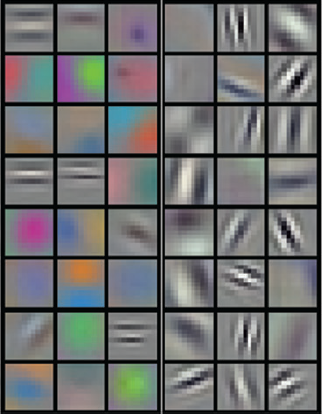
\includegraphics[width=79pt]{figures/sim-real-gabors/alexnet.png} \\
      \scriptsize\parencite{krizhevsky2012imagenet}
    \end{tabular}
  \end{subfigure}
  \begin{subfigure}[b]{0.04\textwidth}
    \raisebox{-\height/2 + 6pt}{
  
\begin{tikzpicture}
    \draw[dashed, gray, ultra thick] (0,0) -- (0,4);
  \end{tikzpicture}
}
  \end{subfigure}
  \begin{subfigure}[b]{0.16\textwidth}
    \setlength{\tabcolsep}{2pt}
    \begin{tabular}{cc}
      \tcbincludegraphics[size=tight,hbox,graphics options={width=\fieldsize}]{figures/sim-real-gabors/ica/1-2d-blob.pdf} &
      \tcbincludegraphics[size=tight,hbox,graphics options={width=\fieldsize}]{figures/sim-real-gabors/ica/2-2d-blob.pdf} \\
      \tcbincludegraphics[size=tight,hbox,graphics options={width=\fieldsize}]{figures/sim-real-gabors/ica/3-2d-blob.pdf} &
      \tcbincludegraphics[size=tight,hbox,graphics options={width=\fieldsize}]{figures/sim-real-gabors/ica/4-2d-blob.pdf} \\
      \tcbincludegraphics[size=tight,hbox,graphics options={width=\fieldsize}]{figures/sim-real-gabors/ica/5-2d-blob.pdf} &
      \tcbincludegraphics[size=tight,hbox,graphics options={width=\fieldsize}]{figures/sim-real-gabors/ica/6-2d-blob.pdf} \\
      \tcbincludegraphics[size=tight,hbox,graphics options={width=\fieldsize}]{figures/sim-real-gabors/ica/7-2d-blob.pdf} &
      \tcbincludegraphics[size=tight,hbox,graphics options={width=\fieldsize}]{figures/sim-real-gabors/ica/8-2d-blob.pdf} \\
      \multicolumn{2}{c}{\scriptsize\parencite{hyvarinen2000independent}}
    \end{tabular}
  \end{subfigure}
  \begin{subfigure}[b]{0.15\textwidth}
    \setlength{\tabcolsep}{2pt}
    \begin{tabular}{cc}
      \tcbincludegraphics[size=tight,hbox,graphics options={width=\fieldsize}]{figures/sim-real-gabors/2d-blobs/1-2d-blob.pdf} &
      \tcbincludegraphics[size=tight,hbox,graphics options={width=\fieldsize}]{figures/sim-real-gabors/2d-blobs/2-2d-blob.pdf} \\
      \tcbincludegraphics[size=tight,hbox,graphics options={width=\fieldsize}]{figures/sim-real-gabors/2d-blobs/3-2d-blob.pdf} &
      \tcbincludegraphics[size=tight,hbox,graphics options={width=\fieldsize}]{figures/sim-real-gabors/2d-blobs/4-2d-blob.pdf} \\
      \tcbincludegraphics[size=tight,hbox,graphics options={width=\fieldsize}]{figures/sim-real-gabors/2d-blobs/5-2d-blob.pdf} &
      \tcbincludegraphics[size=tight,hbox,graphics options={width=\fieldsize}]{figures/sim-real-gabors/2d-blobs/6-2d-blob.pdf} \\
      \tcbincludegraphics[size=tight,hbox,graphics options={width=\fieldsize}]{figures/sim-real-gabors/2d-blobs/7-2d-blob.pdf} &
      \tcbincludegraphics[size=tight,hbox,graphics options={width=\fieldsize}]{figures/sim-real-gabors/2d-blobs/8-2d-blob.pdf} \\
      \multicolumn{2}{c}{\scriptsize\labelcref{item:many-neuron-model} SCM}
    \end{tabular}
  \end{subfigure}
  \caption{
    \textbf{(左)}
    来自非人灵长类动物(NHP)初级视觉皮层的空间感受野(RFs)局部化~\parencite[][图~2]{ringach2002spatial}
    以及来自NHP~\parencite[][图~2]{decharms1998optimizing}和雪貂~\parencite[][图~2]{singer2018sensory}初级听觉皮层的时空感受野(RFs)局部化。
    \textbf{(中)}
    用于ImageNet分类训练的AlexNet的局部化第一层卷积核半切片~\parencite{krizhevsky2012imagenet}。
    \textbf{(右)}
    从任务\cref{sec:task}中学习到的局部化感受野,在二维空间中使用独立成分分析(ICA)~\parencite{hyvarinen2000independent}
    和软委员会机器(SCM;\labelcref{item:many-neuron-model},固定第二层权重)
    来自\cref{sec:model}。
    \emph{局部化——空间和/或时间选择性——在不同的设置中都有出现,
      无论是通过生物系统中的响应最大化(左),还是通过检查人工系统中的线性滤波器(中、右)。}
  }
  \label{fig:sim-real-gabors}
  \vspace{-8pt}
\end{figure}
